% ============================================================
%  CAPÍTULO 3 — DISEÑO METODOLÓGICO
% ============================================================
\chapter{Diseño Metodológico}

En este capítulo se describe la metodología utilizada para implementar el
sistema de detección de \ac{MAP} a partir del análisis de imágenes
multiespectrales aéreas del suelo. El diseño abarca cuatro etapas principales:
(1) construcción de la base de datos, (2) preprocesamiento radiométrico y
geométrico de las imágenes, (3) extracción de características espectrales, y
(4) clasificación y validación. La Figura~\ref{fig:pipeline_general} muestra
el diagrama general del \textit{pipeline} implementado.

\begin{figure}[H]
  \centering
  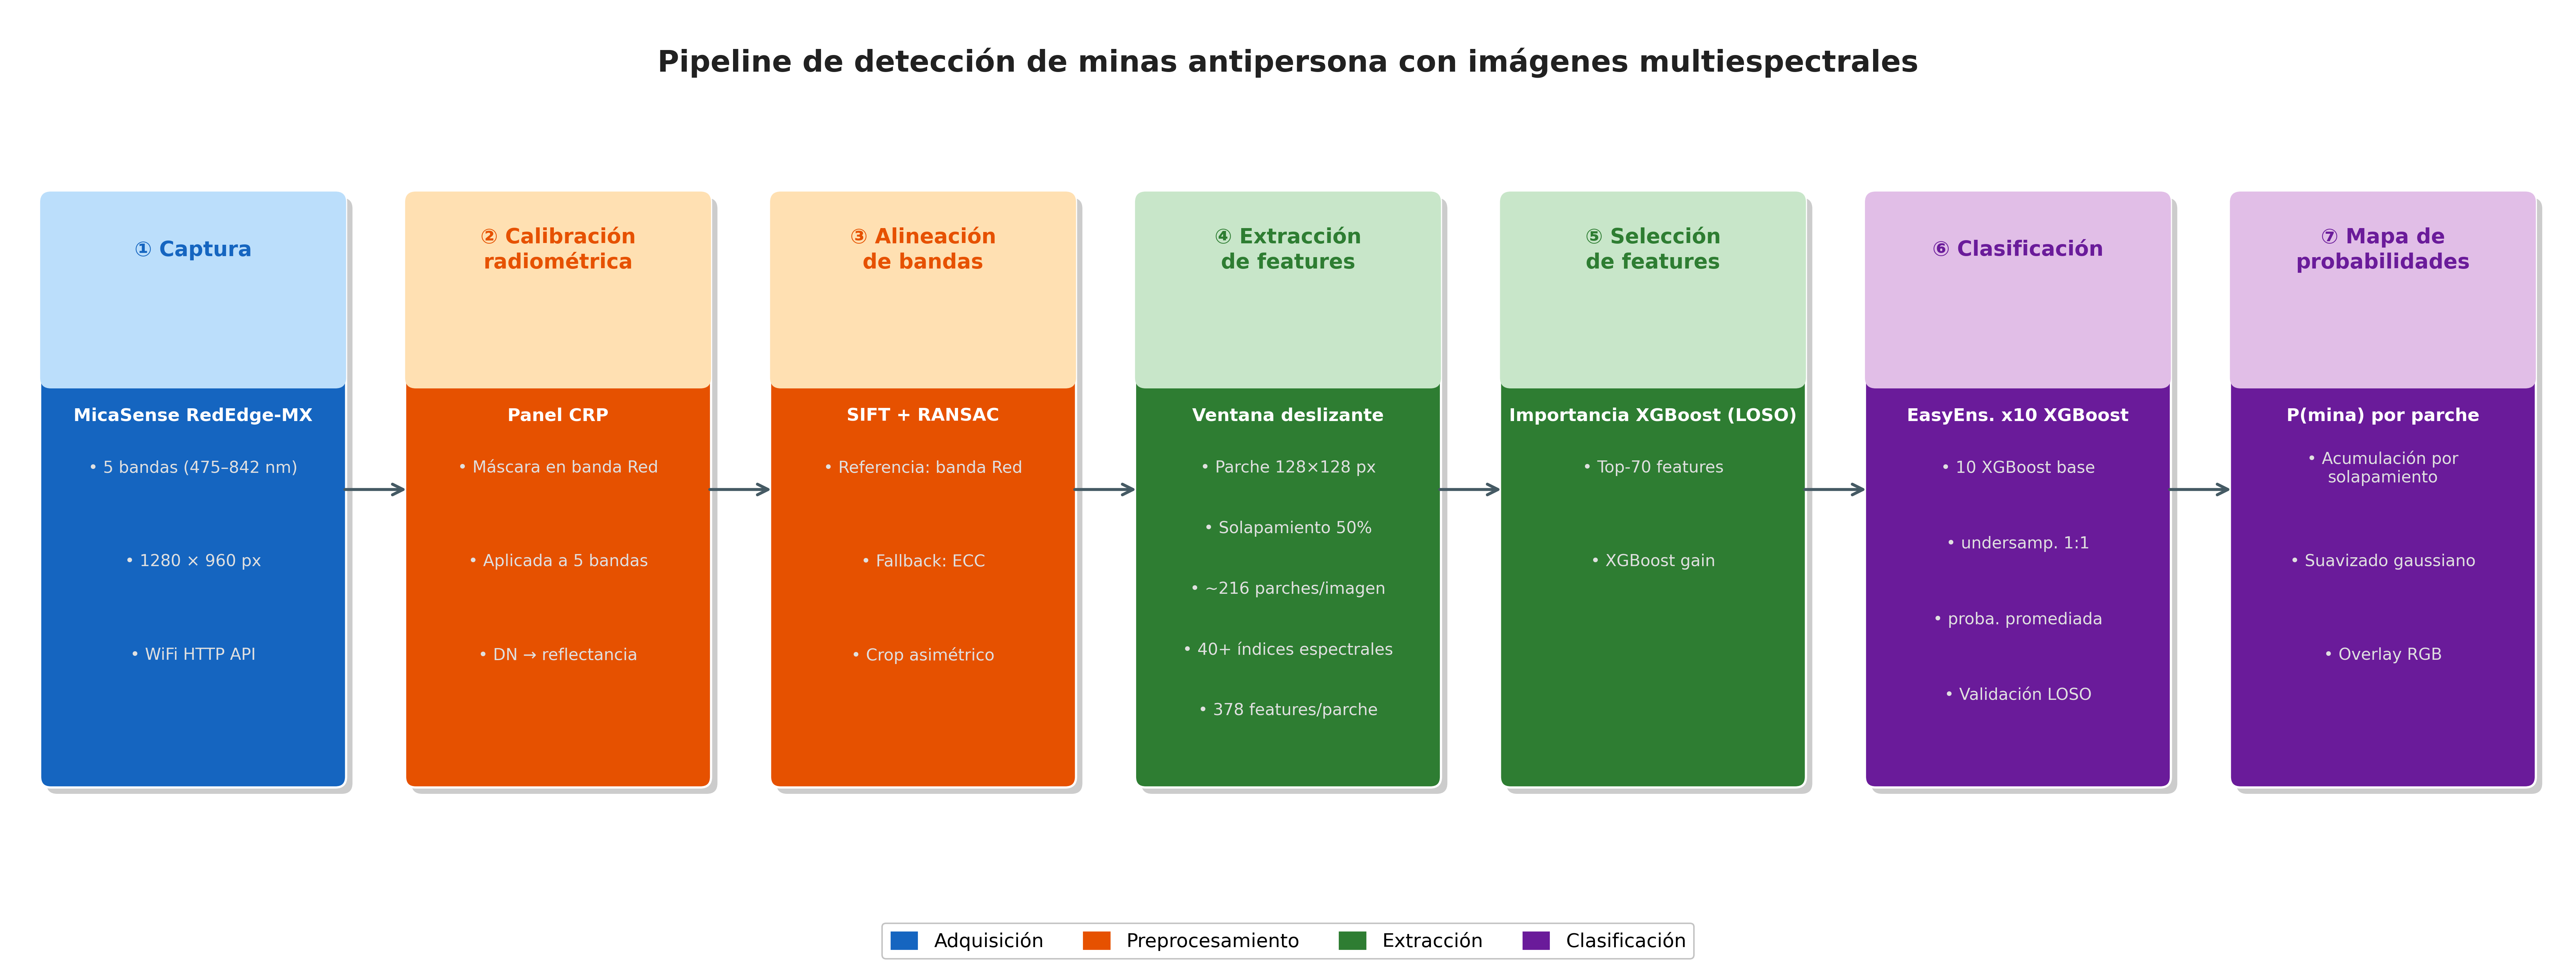
\includegraphics[width=\textwidth]{figuras/pipeline_general.png}
  \caption{Diagrama general del sistema de detección de \ac{MAP} propuesto.
           Las etapas se agrupan en cuatro categorías: adquisición (azul),
           preprocesamiento (naranja), extracción de características (verde)
           y clasificación (morado).}
  \label{fig:pipeline_general}

  {\footnotesize Fuente: elaboración propia.}
\end{figure}

% -------------------------------------------------------------
\section{Diseño del experimento}

\subsection{Construcción de las minas emuladas}

Para garantizar la seguridad durante la experimentación, se construyeron minas
emuladas que replican las características espectrales y morfológicas de las
\ac{MAP} tipo quiebrapatas, sin emplear material explosivo real. Siguiendo la
metodología establecida en \cite{forero2022}, cada mina se fabricó con los
siguientes componentes:

\begin{itemize}
  \item Cilindro externo de \ac{PVC} de \SI{10.2}{cm} de alto y
    \SI{7.62}{cm} de diámetro.
  \item \SI{400}{g} de carbón de antracita, como sustituto seguro del
    \ac{TNT}. La Tabla~\ref{tab:tnt_carbon} resume las propiedades térmicas
    de ambos materiales, evidenciando su similitud en calor específico y
    conductividad térmica \cite{forero2022}.
  \item \SI{20}{g} de clavos de acero, para simular los fragmentos metálicos
    presentes en las minas artesanales colombianas.
  \item Una pila de 9~V en el interior, para simular el sistema de activación
    eléctrico de la mina quiebrapatas real (que emplea una batería de 9~V
    como fuente de energía del detonador eléctrico). Este elemento diferencia
    las minas emuladas de este trabajo respecto al trabajo previo del grupo
    \ac{PSI} \cite{forero2022}, donde el detonador no incluía batería.
\end{itemize}

\begin{table}[H]
\centering
\caption{Propiedades térmicas del \ac{TNT} y del carbón de antracita \cite{forero2022}}
\label{tab:tnt_carbon}
\begin{tabular}{lcc}
\toprule
\textbf{Propiedad} & \textbf{TNT} & \textbf{Carbón de antracita} \\
\midrule
Densidad (\si{g/cm^3})             & 1.56 & 1.37 \\
Calor específico (\si{J/(g\cdot K)})   & 1.37 & 1.26 \\
Conductividad térmica (\si{W/(m\cdot K)}) & 0.26 & 0.23 \\
\bottomrule
\end{tabular}

  {\footnotesize Fuente: elaboración propia.}
\end{table}

El uso del carbón de antracita como sustituto del \ac{TNT} responde a dos
criterios. \textbf{Térmicamente}, sus propiedades similares de densidad, calor
específico y conductividad térmica lo hacen idóneo para replicar el contraste
infrarrojo de la mina real, siguiendo la metodología de los trabajos previos del
grupo \ac{PSI} \cite{forero2022,tenorio2024}. \textbf{Espectralmente}, el carbón
de antracita presenta baja reflectancia en el rango visible e infrarrojo cercano
sin características distintivas que puedan confundirse con la vegetación
\cite{barnawi2022}, lo que implica que el sistema no detecta el carbón directamente
sino las anomalías espectrales que su presencia induce en el suelo y la vegetación
circundantes --- el mecanismo en que se fundamenta la detección.

El mecanismo de activación se emula mediante una jeringa de \SI{5}{mL}
insertada en la tapa superior del cilindro. Al momento del enterramiento,
la cabeza del émbolo queda expuesta sobre la superficie del suelo ---
funcionalmente, es la parte que se pisa para activar la mina real ---,
por lo que en la base de datos definitiva se cubre con hojas u otro material
vegetal del entorno para evitar que sea visualmente distinguible desde la
cámara. Esta decisión de diseño fue determinante para la base de datos definitiva,
como se describe en la Sección~\ref{sec:iteracion_previa}.

La Figura~\ref{fig:minas_simuladas} muestra las minas emuladas construidas
para este experimento, con vista lateral y superior.

\begin{figure}[H]
  \centering
  \begin{subfigure}[b]{0.40\textwidth}
    \centering
    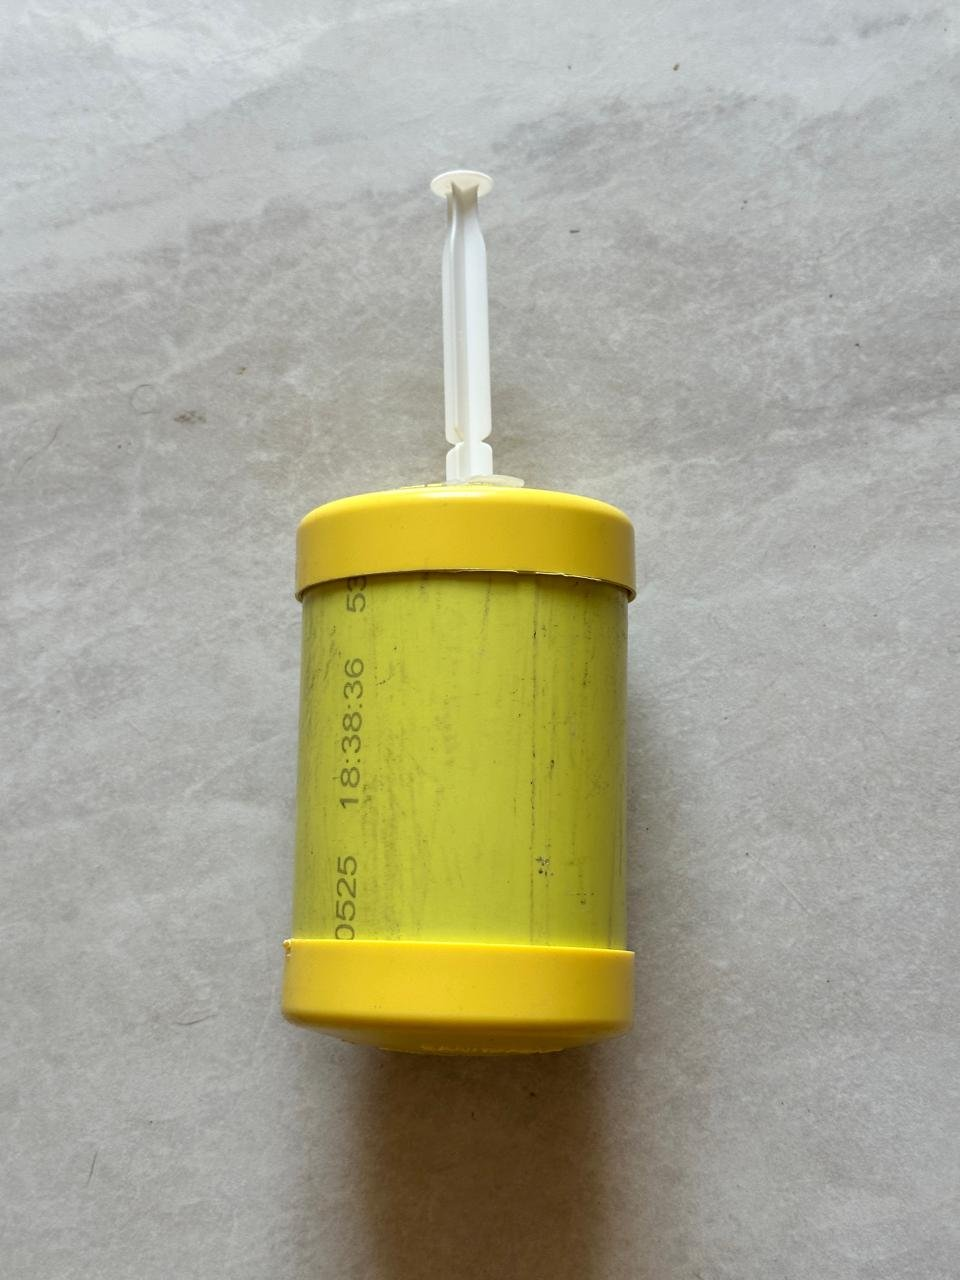
\includegraphics[height=6cm]{figuras/mina_lateral.png}
    \caption{Vista lateral}
  \end{subfigure}
  \hspace{1cm}
  \begin{subfigure}[b]{0.40\textwidth}
    \centering
    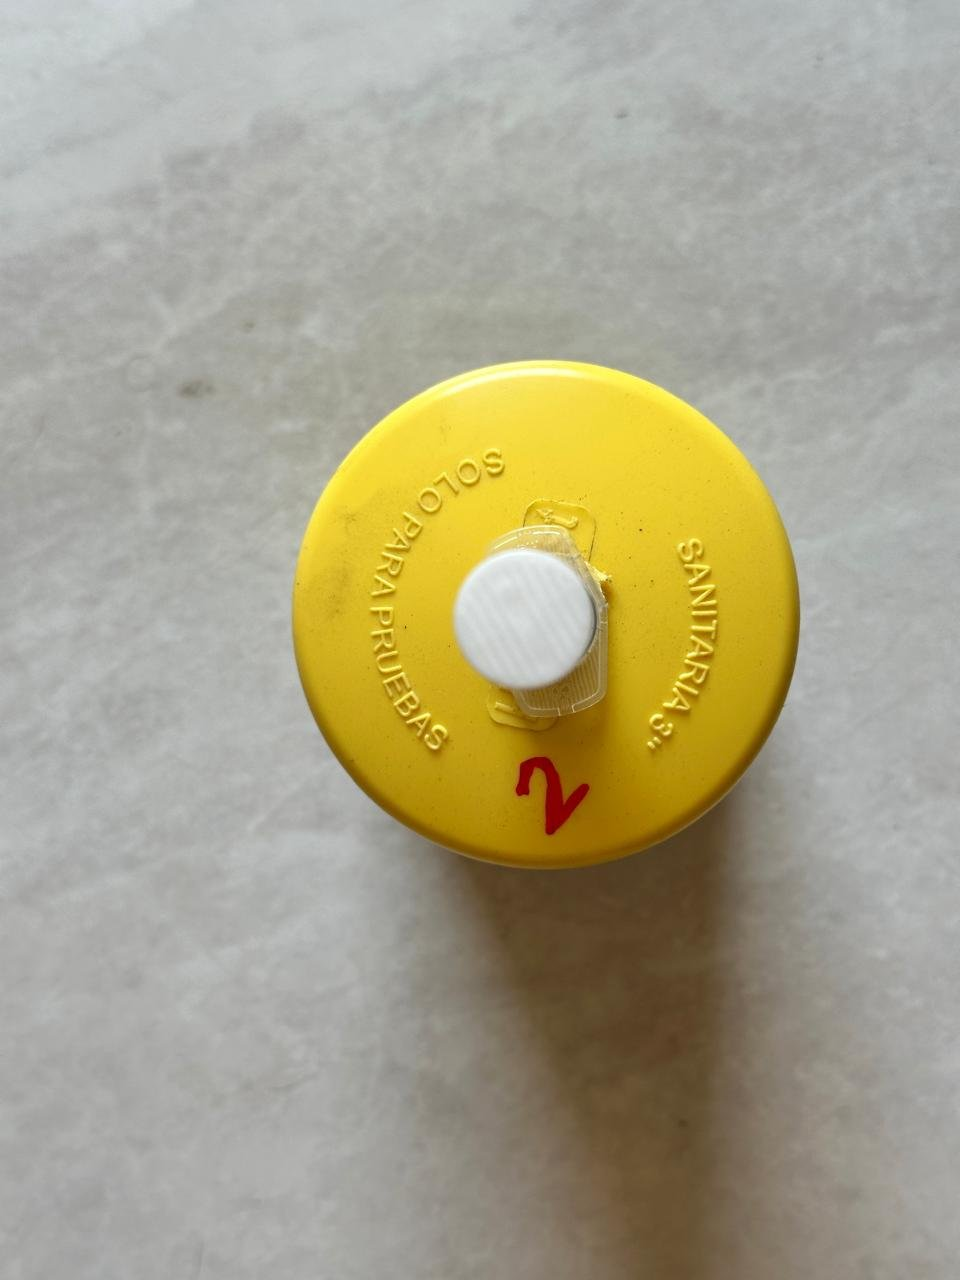
\includegraphics[height=6cm]{figuras/mina_superior.png}
    \caption{Vista superior (tapa con cabeza de émbolo expuesta)}
  \end{subfigure}
  \caption{Mina emulada tipo quiebrapatas construida para el experimento.
           Cilindro de \ac{PVC} con carbón de antracita, clavos y pila de 9~V
           en su interior. La cabeza del émbolo de la jeringa queda expuesta
           sobre la superficie del suelo; en la base de datos definitiva se cubre
           con hojas del entorno para evitar su detección trivial.}
  \label{fig:minas_simuladas}

  {\footnotesize Fuente: elaboración propia.}
\end{figure}

\subsection{Objetos de interferencia (potenciales falsos positivos)}
\label{sec:objetos_interferencia}

Con el propósito de dotar al experimento de mayor realismo, en cada zona de
mina se dispusieron tres objetos de interferencia \textbf{enterrados a la
misma profundidad que la mina correspondiente}, a \SI{20}{cm} de distancia
del centro: una roca a la izquierda, una botella de vidrio en la parte
superior y una lata de aluminio a la derecha. Esta distribución se mantuvo
constante en todas las zonas  con mina y sesiones (véase Figura~\ref{fig:disposicion_zona}).

Cada zona de captura cubre un área de aproximadamente \SI{60}{cm} $\times$
\SI{60}{cm}, con la mina ubicada en el centro geométrico de la subárea.
Los objetos de interferencia quedan a los lados, dentro del campo de visión
de la cámara pero fuera de la región central donde se concentra la firma
espectral de la mina.

La selección de estos objetos responde a dos criterios. Primero, todos ellos
aparecen en contextos reales de terrenos minados: rocas y objetos metálicos
son comunes en zonas rurales colombianas. Segundo, y más importante para el
diseño experimental, cada objeto puede generar anomalías espectrales que
el clasificador podría confundir con una \ac{MAP}:

\begin{itemize}
  \item \textbf{Roca:} su composición mineralógica diferente al suelo circundante
    genera una firma espectral distinta en las bandas Roja y Red Edge,
    potencialmente similar a la perturbación del suelo sobre una mina.
  \item \textbf{Botella de vidrio:} su alta reflectancia en el espectro visible
    genera valores anómalos en índices como \ac{VARI} y \ac{NDRB},
    similares a los producidos por suelo perturbado.
  \item \textbf{Lata de aluminio:} los metales tienen reflectancia muy alta y
    relativamente plana en todas las bandas, generando valores atípicos en
    índices que involucran ratios entre bandas visibles e infrarrojas.
\end{itemize}

El análisis de qué fracción de los falsos positivos se asocia a estos
objetos se presenta en la Sección~\ref{sec:analisis_fp}.

\begin{figure}[H]
  \centering
  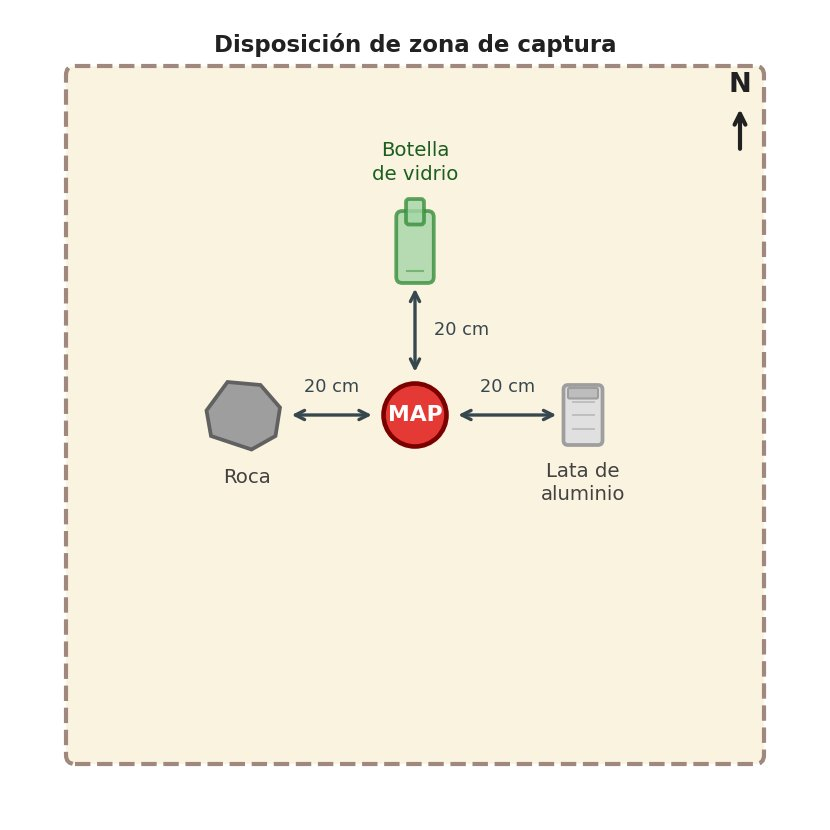
\includegraphics[width=0.45\textwidth]{figuras/disposicion_zona.png}
  \caption{Esquema de disposición de la mina emulada y los objetos de
           interferencia en cada zona de captura (\SI{60}{cm} $\times$ \SI{60}{cm}).
           La \ac{MAP} se ubica en el centro; la roca a la izquierda, la
           botella de vidrio en la parte superior y la lata de aluminio a
           la derecha, todos enterrados a la misma profundidad que la mina
           y a \SI{20}{cm} del centro.}
  \label{fig:disposicion_zona}

  {\footnotesize Fuente: elaboración propia.}
\end{figure}


\subsection{Descripción del terreno experimental}

El experimento se llevó a cabo en un área verde del campus de la Universidad
del Valle, sede Meléndez, en Santiago de Cali. El terreno seleccionado
presenta suelo con predominio de textura arenosa y vegetación limitada,
compuesta principalmente por gramíneas y plantas herbáceas de hoja ancha. La zona está rodeada por árboles de mediano y gran porte y
tiene una edificación adyacente, lo que genera condiciones de sombra
parcial en horas de la mañana temprana.

El área total del terreno experimental es de aproximadamente
\textbf{\SI{10}{m} $\times$ \SI{6}{m}}. La Figura~\ref{fig:terreno} muestra
el área de trabajo: la vista general antes del experimento y la disposición
de las zonas delimitadas con cinta de señalización amarilla durante una
sesión de campo.

\begin{figure}[H]
  \centering
  \begin{subfigure}[b]{0.48\textwidth}
    \centering
    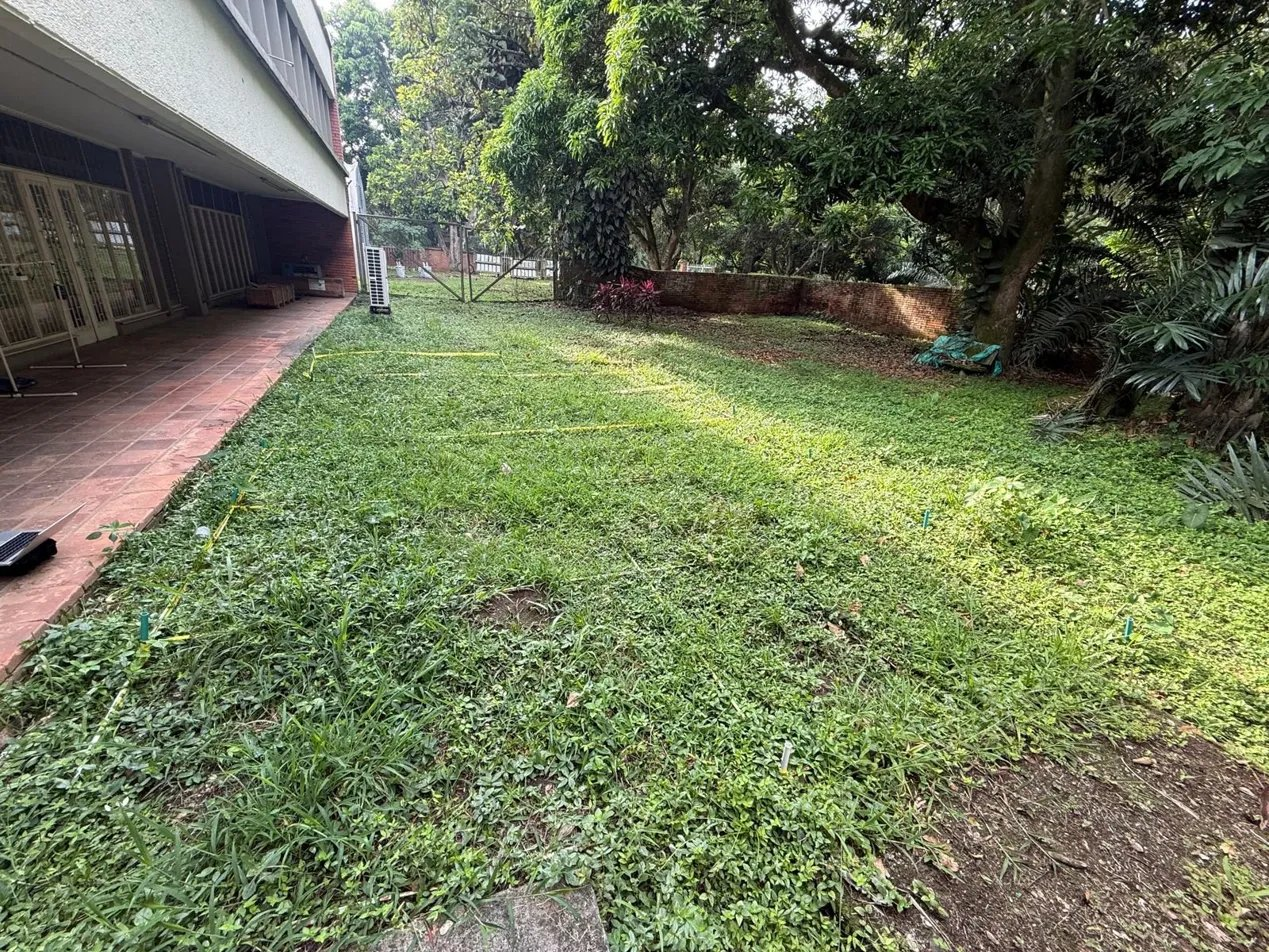
\includegraphics[width=\textwidth]{figuras/terreno_general.png}
    \caption{Vista general del área experimental}
  \end{subfigure}
  \hfill
  \begin{subfigure}[b]{0.48\textwidth}
    \centering
    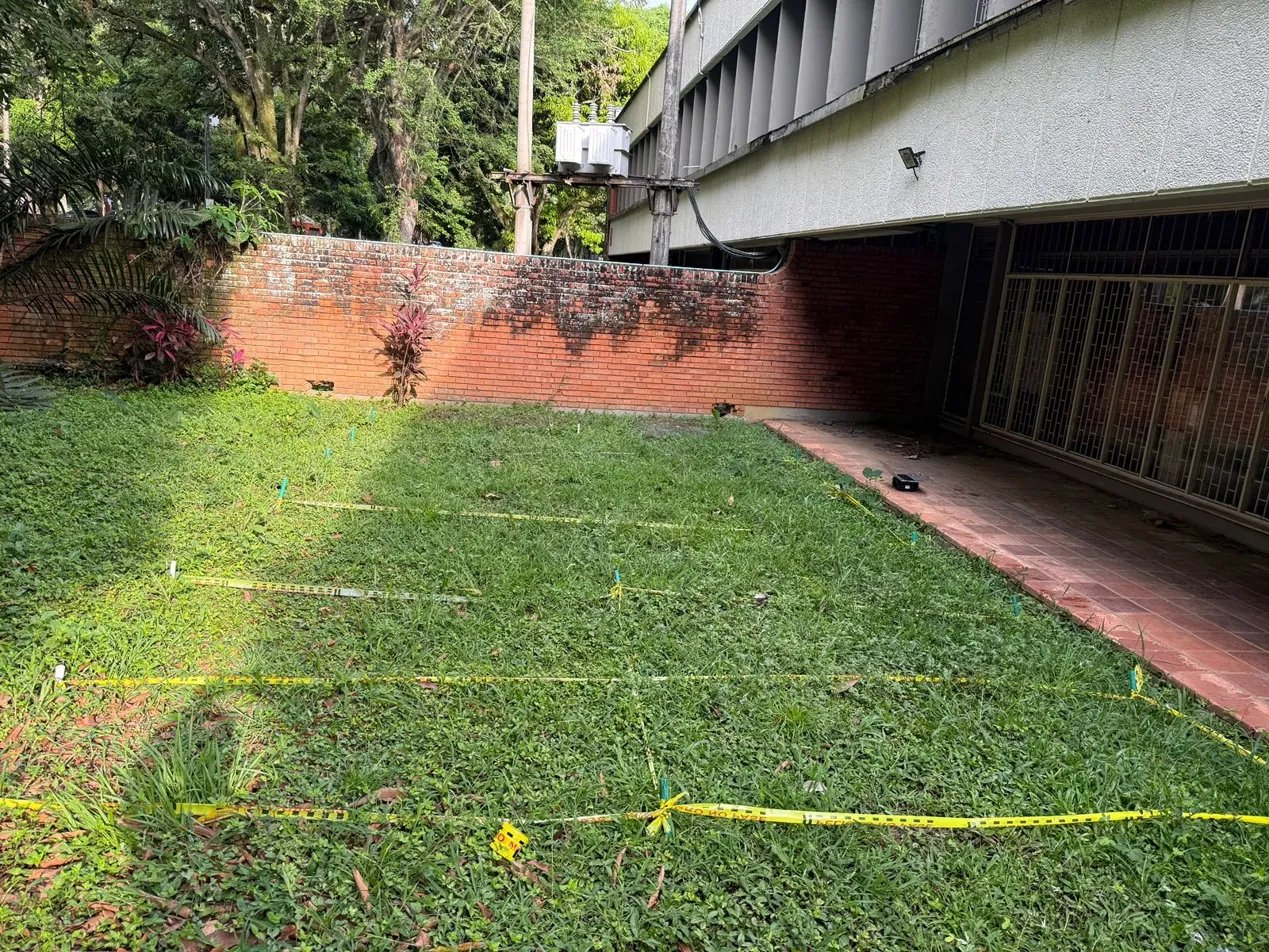
\includegraphics[width=\textwidth]{figuras/terreno_delimitado.png}
    \caption{Zonas delimitadas con cinta de señalización}
  \end{subfigure}
  \caption{Terreno experimental en el campus de la Universidad del Valle,
           sede Meléndez. (a) Vista general con cobertura vegetal limitada, rodeada por árboles de mediano y gran porte y una
           edificación adyacente. (b) Distribución de las doce zonas de
           captura delimitadas con estacas y cinta amarilla.}
  \label{fig:terreno}

  {\footnotesize Fuente: elaboración propia.}
\end{figure}

Previo al inicio del experimento se realizó una poda completa de la
vegetación en toda el área de trabajo con el propósito de homogenizar
las condiciones iniciales y garantizar vegetación limitada, en concordancia
con el objetivo específico~1 del presente trabajo. A partir de ese momento
no se realizó ninguna intervención adicional, permitiendo el crecimiento
natural de la vegetación durante todo el período experimental. Las minas
llevan aproximadamente seis meses enterradas desde el inicio del
experimento, tiempo suficiente para que los efectos crónicos del
enterramiento ---perturbación del suelo y posible estrés vegetal
diferencial--- se hayan desarrollado progresivamente. Un aspecto favorable
de este diseño es que la vegetación cubre completamente las zonas de mina,
haciendo que los artefactos sean invisibles a simple vista, simulando
fielmente el camuflaje natural de las \ac{MAP} en entornos reales.

Para garantizar la altura y verticalidad de la captura con precisión y
reproducibilidad entre sesiones, se diseñó e implementó una estructura de
soporte fabricada en tubo de \ac{PVC} que posiciona la cámara a exactamente
\SI{1}{m} sobre cada zona (véase Sección~\ref{sec:montaje}). Esta solución
podría ser reemplazada en trabajos futuros por un \ac{UAV} volando a dicha
altura, lo que permitiría escalar el sistema a áreas de mayor extensión.



\subsection{Distribución de zonas}

El área experimental de \SI{10}{m} $\times$ \SI{6}{m} se subdividió en
doce zonas de captura distribuidas en una matriz de $6 \times 2$, como
se muestra en la Figura~\ref{fig:distribucion_zonas}.

\begin{figure}[H]
  \centering
  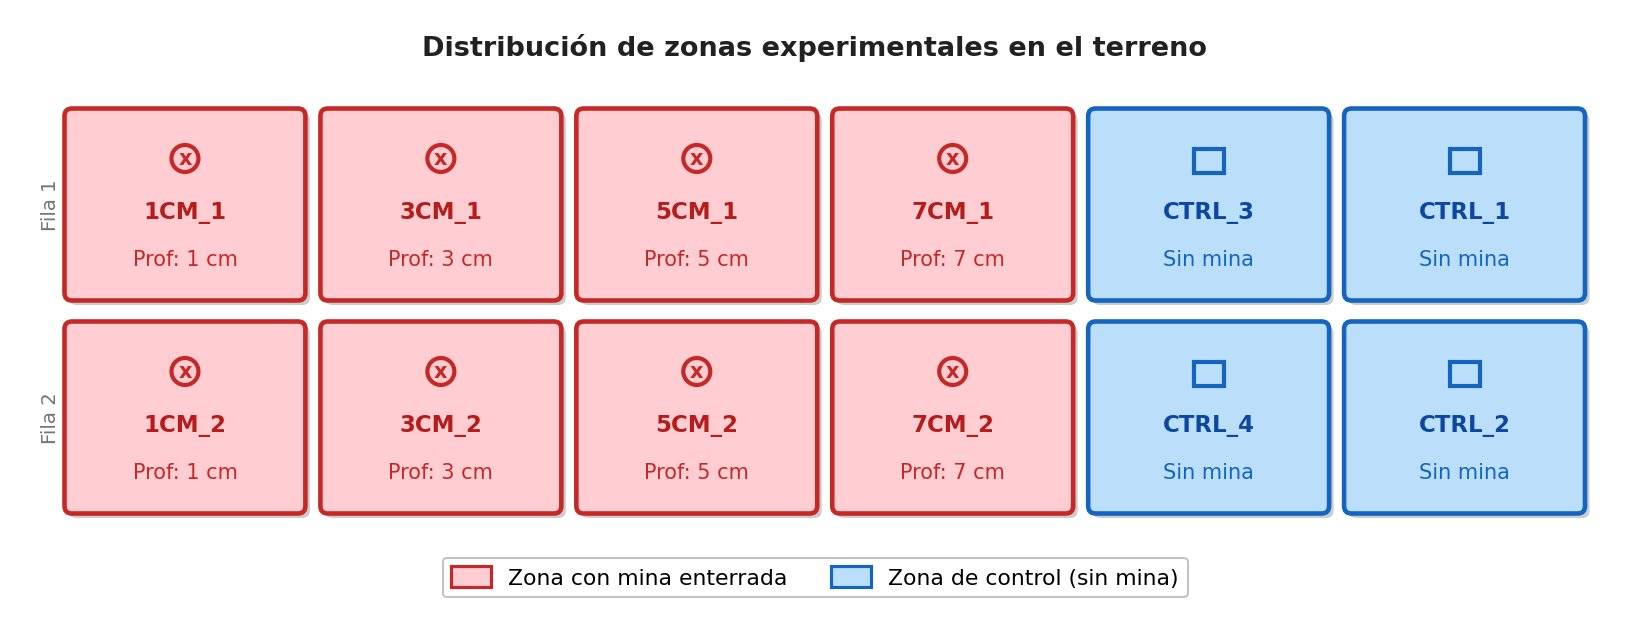
\includegraphics[width=0.95\textwidth]{figuras/distribucion_zonas.png}
  \caption{Distribución de las doce zonas de captura en el área experimental
         de \SI{10}{m} $\times$ \SI{6}{m}, organizadas en una matriz de
         $6 \times 2$. Cada zona cubre \SI{60}{cm} $\times$ \SI{60}{cm},
         con la \ac{MAP} emulada ubicada en el centro geométrico. Las zonas
         rojas contienen \ac{MAP} enterradas a distintas profundidades; las
         azules son de control (sin mina). Cada zona de mina incluye además
         tres objetos de interferencia enterrados a la misma profundidad
         (véase Sección~\ref{sec:objetos_interferencia}).}
  \label{fig:distribucion_zonas}

  {\footnotesize Fuente: elaboración propia.}
\end{figure}

Cada zona fue delimitada con estacas y cinta de señalización amarilla
para garantizar la reproducibilidad de la posición de captura entre sesiones.
A partir de la Sesión~3 se incorporaron cuatro zonas de control por sesión
(relación 2:1 respecto a las zonas de mina), frente a la única zona de control
de la Sesión~2 (relación 8:1), con el fin de reducir el desbalance de clases
en el conjunto de entrenamiento.



\subsection{Iteración previa del diseño experimental}
\label{sec:iteracion_previa}

Antes de constituir la base de datos definitiva, se realizó una fase experimental
previa que fue descartada en su totalidad. En esa iteración, las minas
emuladas se enterraban dejando la cabeza del émbolo de la jeringa completamente blanco expuesta
sobre la superficie del terreno durante las capturas, sin cubrirla. Este
elemento de color blanco intenso generaba una firma espectral trivialmente
discriminable: algoritmos de segmentación básicos como k-means identificaban
la zona de la mina con casi el 100\,\% de exactitud, no por detectar la
perturbación del suelo o el estrés vegetal asociados a la mina enterrada,
sino por detectar el color blanco del émbolo en la imagen de espectro visible.

La detección del émbolo visible no constituye una solución al problema
planteado --- en una situación real, las \ac{MAP} probablemente no presentarían elementos
tan contrastantes en superficie --- por lo que se tomó la decisión de reiniciar
la base de datos completa, cubriendo los émbolos con hojas u otro material vegetal
del entorno antes de cada captura, de modo que las minas emuladas no tuvieran
ningún elemento visible que facilitara su localización trivial. Esta decisión
está alineada con el objetivo de detectar anomalías espectrales sutiles del
suelo y la vegetación, no elementos superficiales de alta reflectancia.

Las imágenes de la iteración previa se conservan como registro, pero no
se utilizan en ninguna etapa del análisis presentado en este trabajo.

% -------------------------------------------------------------
\section{Protocolo de adquisición de imágenes}

\subsection{Sistema de soporte de la cámara}
\label{sec:montaje}

Para garantizar la altura de captura con precisión y reproducibilidad entre
sesiones, se diseñó y construyó un sistema de soporte estacionario fabricado
en tubo de \ac{PVC}, con forma de pórtico en H, que posiciona la cámara a
exactamente \SI{1}{m} sobre cada zona de captura
(véase Figura~\ref{fig:soporte}). Esta solución permitió controlar con
precisión la altura y la verticalidad de la cámara, condiciones difíciles
de garantizar en vuelo libre. En el futuro, la misma metodología podría
aplicarse montando la cámara en un \ac{UAV} volando a dicha altura, lo
que permitiría escalar el sistema a áreas de mayor extensión.

% \begin{figure}[H]
%   \centering
%   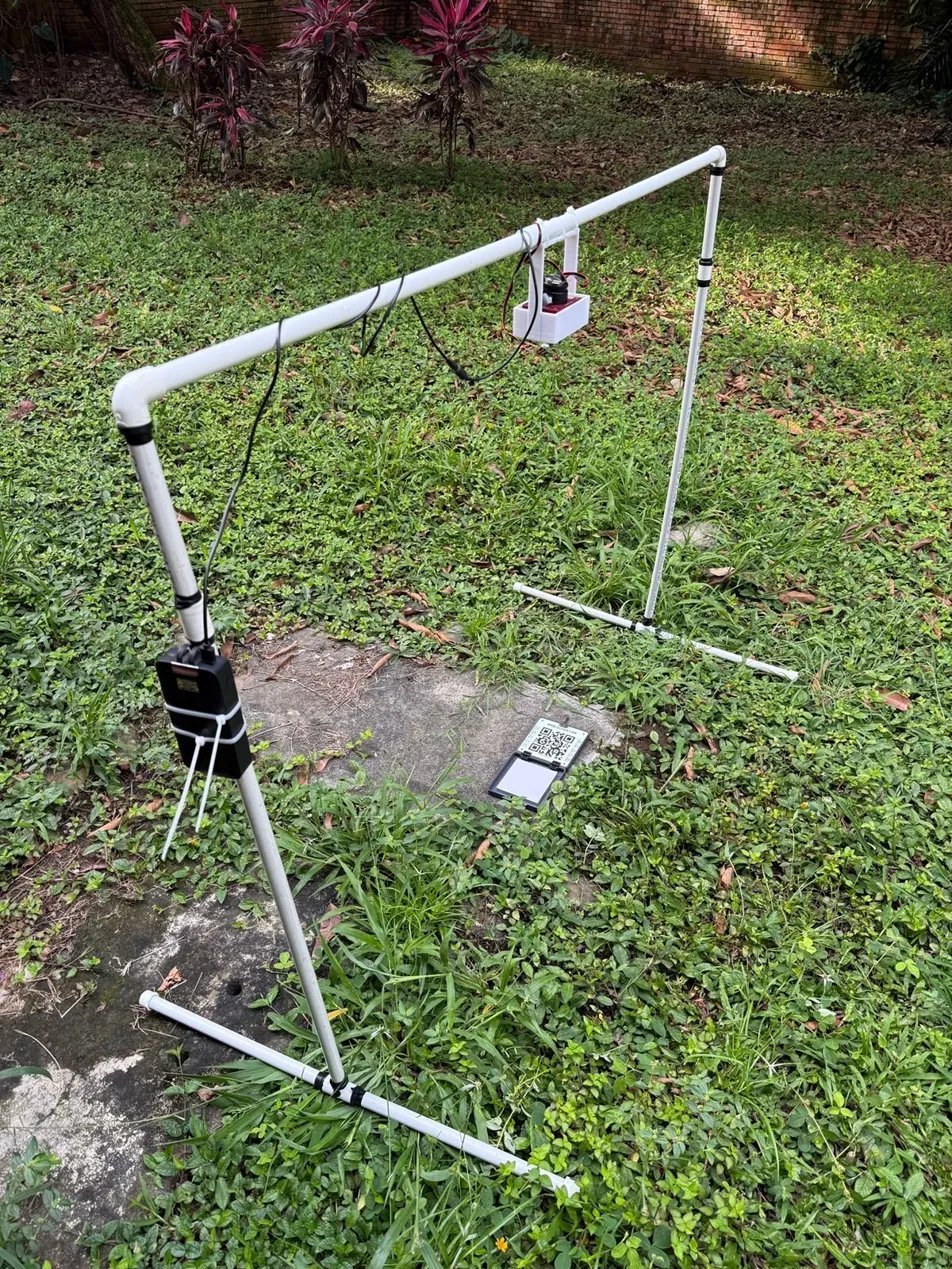
\includegraphics[width=0.7\textwidth]{figuras/soporte_pvc.jpg}
%   \caption{Sistema de soporte de la cámara MicaSense RedEdge-MX.
%            Estructura de tubo PVC con soporte impreso en 3D (color morado)
%            para fijar la cámara en posición nadir a \SI{1}{m} de altura.}
%   \label{fig:soporte}
% \end{figure}

La cámara MicaSense RedEdge-MX se fija en el extremo horizontal del pórtico
mediante un soporte fabricado en impresión 3D, apuntando en posición nadir
(perpendicular al suelo). La Figura~\ref{fig:soporte} muestra el sistema completo
durante una sesión de campo, con el panel de calibración de reflectancia
visible en el suelo. La altura se verificó con un metro desde el nivel
del suelo hasta los lentes de la cámara, con un margen de error de
$\pm$\SI{3}{cm}. La verticalidad del soporte se comprobó con un nivel de
burbuja antes de cada captura. La estructura se desplazó manualmente de zona
en zona, reposicionándose sobre el centro de cada área delimitada.

\begin{figure}[H]
  \centering
  \begin{subfigure}[b]{0.52\textwidth}
    \centering
    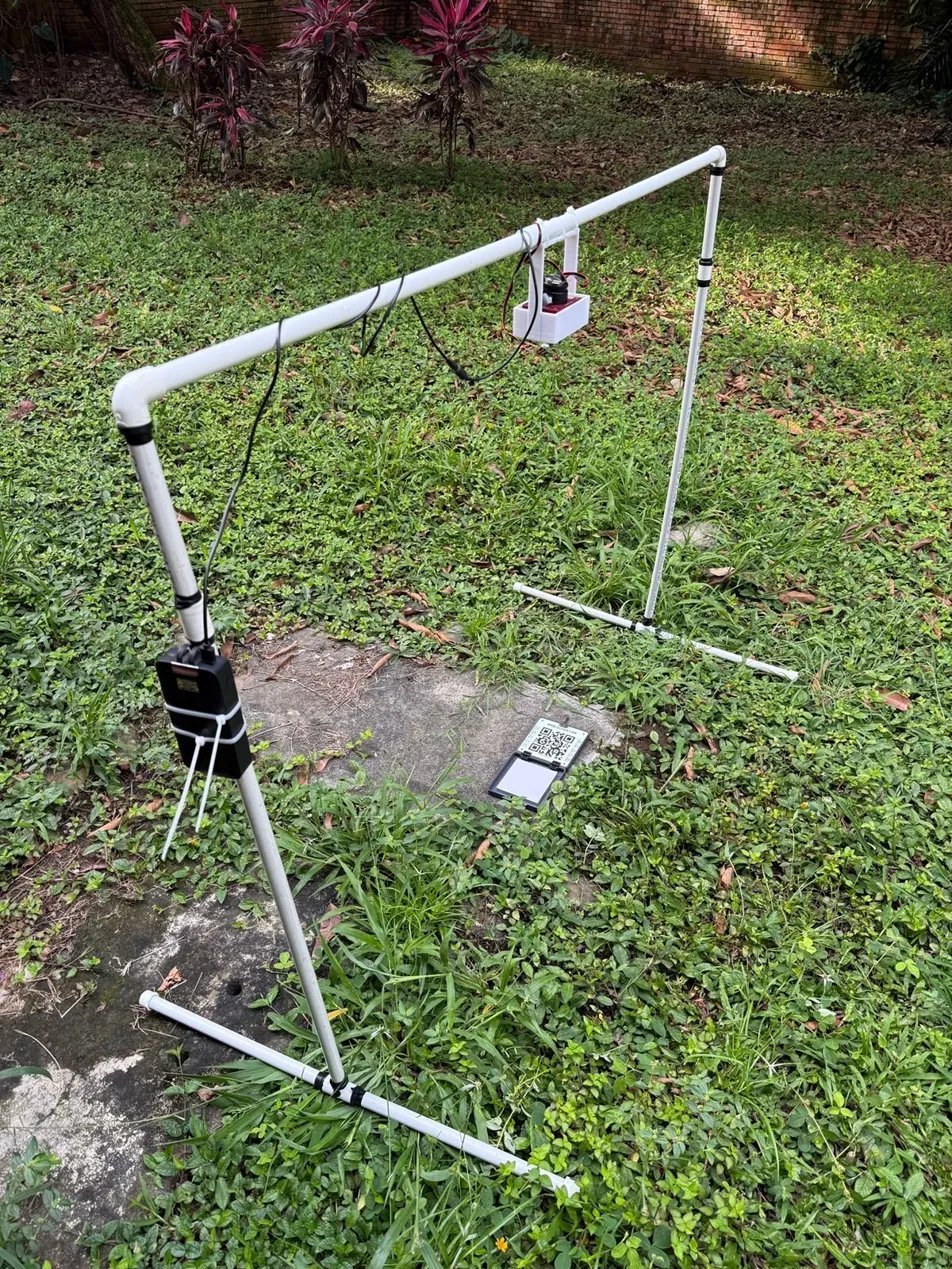
\includegraphics[width=\textwidth]{figuras/soporte_pvc.png}
    \caption{Sistema de soporte en pórtico de \ac{PVC} con la cámara
             en posición nadir. El panel \ac{CRP} se observa en el suelo.}
  \end{subfigure}
  \hfill
  \begin{subfigure}[b]{0.42\textwidth}
    \centering
    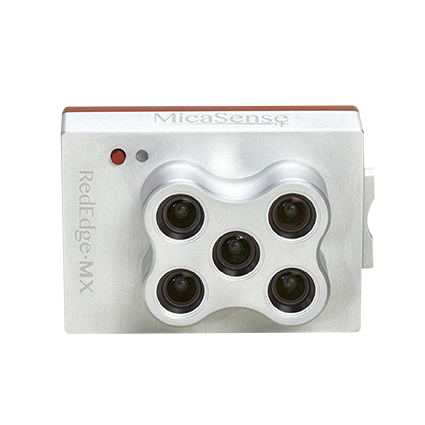
\includegraphics[width=\textwidth]{figuras/micasense_rededge.png}
    \caption{Cámara MicaSense RedEdge-MX con sus cinco lentes
             correspondientes a las bandas Blue, Green, Red,
             Red Edge y NIR.}
  \end{subfigure}
  \caption{Equipo de captura multiespectral utilizado en el experimento.}
  \label{fig:soporte}

  {\footnotesize Fuente: (a) elaboración propia; (b) tomado de \url{https://al-top.com/producto/micasense-rededge-mx/}.}
\end{figure}

La elección de un sistema estacionario, aunque limita la movilidad en
comparación con un \ac{UAV}, ofrece ventajas para este experimento: permite
tiempos de captura más largos por zona, elimina la inestabilidad posicional
causada por el viento que afecta a los drones a baja altura, y garantiza
una altura de adquisición más consistente.

\subsection{Condiciones ambientales}

Las condiciones meteorológicas durante cada sesión de campo se registraron
a partir de la estación meteorológica de la Universidad del Valle, ubicada
en las proximidades del área de experimentación. Las variables registradas
fueron: irradiancia solar global (\si{W/m^2}), temperatura del aire
(\si{\celsius}), humedad relativa (\%), precipitación acumulada en las
24~horas previas (\si{mm}) y cobertura nubosa estimada. La
Tabla~\ref{tab:condiciones_ambientales} resume estas condiciones para cada
sesión de captura.

\begin{table}[H]
\centering
\caption{Condiciones ambientales registradas por sesión de captura}
\label{tab:condiciones_ambientales}
\begin{tabular}{ccccccc}
\toprule
\textbf{Sesión} & \textbf{Fecha} & \textbf{Hora} & \textbf{Rad. solar (\si{W/m^2})} &
\textbf{Temp. (\si{\celsius})} & \textbf{HR (\%)} & \textbf{Precip. 24h (\si{mm})} \\
\midrule
S1            & 16 abr. & 09:44 & 620.0 & 22.4 & 90.5 & 8.0 \\
S2            & 16 abr. & 13:10 & 778.7 & 26.4 & 72.8 & 5.2 \\
S3            & 23 abr. & 12:34 & 346.7 & 28.2 & 60.7 & 0.0 \\
S4            & 24 abr. & 17:21 &  64.5 & 27.5 & 61.8 & 0.0 \\
S5            & 30 abr. & 17:17 &  73.3 & 29.2 & 63.6 & 0.0 \\
S6            & 07 may. & 07:30 & 161.5 & 23.6 & 84.5 & 0.0 \\
S7            & 07 may. & 16:40 & 143.9 & 29.1 & 65.5 & 0.0 \\
\bottomrule
\multicolumn{7}{l}{\small Todas las sesiones en 2026. S6 y S7 fueron capturadas el mismo día en horarios distintos.} \\
\multicolumn{7}{l}{\small S1: HR=90.5\,\% y precipitación previa de 8.0~mm; no forma parte de la base de datos oficial (S2--S7).}
\end{tabular}

  {\footnotesize Fuente: elaboración propia.}
\end{table}

Las condiciones ambientales registradas evidencian la variabilidad presente
en la base de datos. La Sesión~2 fue capturada a las 13:10 con HR~=~72.8\,\%
y precipitación previa de 5.2~mm. Las sesiones S3 a S5 registraron
HR~$\approx$~61\,\% y precipitación nula en las 24~h previas. La Sesión~6
fue capturada a las 07:30 con HR~=~84.5\,\% y ángulo solar rasante. La base
de datos oficial comprende las sesiones S2--S7; la Sesión~1 se excluyó de
ella. Sus condiciones atípicas ---captura a las 09:44 con posible rocío
(HR~=~90.5\,\%, precipitación previa de 8.0~mm) y una sola zona de control
disponible--- degradaron la señal hasta un AUC~$\approx$~0.47 como fold de
prueba, por debajo del nivel de azar. Más que un dato descartable, la
Sesión~1 establece empíricamente un \textbf{límite operativo} del enfoque: la
alta humedad superficial satura la respuesta espectral pasiva. Por ello se
excluye del protocolo oficial (S2--S7) y se retoma como limitación en el
Capítulo~\ref{cap:conclusiones}.

\subsection{Procedimiento de captura}

Para cada sesión de campo, el procedimiento de captura siguió los pasos:

\begin{enumerate}
\item \textbf{Captura del panel de calibración al inicio.} Antes de
  recorrer las zonas, se capturó una imagen del Panel de Reflectancia
  Calibrada (\ac{CRP}) bajo iluminación directa de sol, con la cámara
  apuntando en posición nadir (perpendicular al suelo, apuntando
  verticalmente hacia abajo) sobre el panel dispuesto horizontalmente
  en el suelo, en un área adyacente a la matriz experimental
  (Figura~\ref{fig:panel_crp}).

\begin{figure}[H]
  \centering
  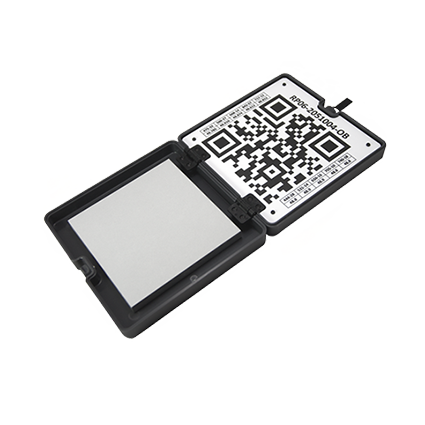
\includegraphics[width=0.40\textwidth]{figuras/panel_crp.png}
  \caption{Panel de Reflectancia Calibrada (\ac{CRP}) de MicaSense
           utilizado para la calibración radiométrica. Sus valores de
           albedo conocidos (Blue: 0.490, Green: 0.491, Red: 0.491,
           Red Edge: 0.488, NIR: 0.490) permiten convertir los valores
           digitales de cada banda a reflectancia absoluta.}
  \label{fig:panel_crp}

  {\footnotesize Fuente: tomado de \url{https://www.airclip.de/MicaSense-Calibrated-Reflectance-Panel-V2}.}
\end{figure}

  \item \textbf{Captura por zona.} El soporte de \ac{PVC} se posicionó sobre
    el centro de cada zona, se verificó la altura y la verticalidad
    mediante nivel de burbuja, y se capturaron las cinco bandas
    simultáneamente. El recorrido siguió un orden fijo de derecha a
    izquierda en zigzag: primero las zonas de control
    (CTRL\_1, CTRL\_2, CTRL\_3, CTRL\_4) y luego las zonas de mina en
    orden decreciente de profundidad (7CM\_1, 7CM\_2, 5CM\_1, 5CM\_2,
    3CM\_1, 3CM\_2, 1CM\_1, 1CM\_2), repitiéndose idéntico en cada sesión.
  \item \textbf{Criterio de iluminación uniforme.} Antes de capturar cada
    zona se verificó que toda el área estuviera bajo la misma condición de luz
    —completamente iluminada o completamente en sombra—, evitando capturas
    con sombras parciales que introducirían gradientes espectrales
    artificiales. Las sombras proyectadas por el edificio adyacente en
    determinadas horas constituían el principal riesgo de incumplimiento
    de este criterio; por ello fue un factor considerado en la selección
    del horario de captura.
  \item \textbf{Captura del Panel de Reflectancia Calibrada al final.}
  Al concluir el recorrido de todas las zonas se repite la captura del
  Panel de Reflectancia Calibrada (\ac{CRP}), para verificar que las
  condiciones de iluminación se mantuvieron estables durante toda la
  sesión y para detectar posibles cambios en las condiciones de iluminación
  comparando los valores de reflectancia del panel al inicio y al final de
  la sesión.
\end{enumerate}

\textbf{Criterio de horario.} Las sesiones S2--S7 se capturaron en distintas
franjas horarias ---mediodía, tarde y mañana temprana--- para
evaluar la estabilidad del sistema ante variaciones de iluminación. El
criterio mínimo aplicado fue evitar capturas con humedad muy alta o
precipitación reciente: la Sesión~1, realizada a las 09:44 con
HR~=~90.5\,\% y precipitación previa de 8.0~mm, produjo firmas espectrales
que se apartaron significativamente del patrón del resto de sesiones, lo que
motivó su exclusión de la base de datos oficial.

\subsection{Estructura de archivos}

Cada captura genera cinco archivos TIFF (uno por banda), nombrados
\texttt{cap\_0001\_band1.tif} a \texttt{cap\_0001\_band5.tif}, organizados
según la siguiente jerarquía:

\begin{lstlisting}[language=bash, caption={Estructura del conjunto de datos}, label={lst:estructura}]
FINAL_DATASET/
+-- SESION_N/
|   +-- PANEL_INICIO/        # 5 TIF (panel al inicio)
|   +-- MINA_1CM_1/          # 5 TIF por zona
|   +-- MINA_3CM_1/ ...
|   +-- ZONA_CONTROL/ ...
|   +-- PANEL_FINAL/         # 5 TIF (panel al final)
|   +-- PROCESADAS/          # generado por el pipeline
|       +-- *_calibrado.tif
|       +-- features_dataset.csv
+-- features_combinado.csv   # todas las sesiones combinadas
\end{lstlisting}

% -------------------------------------------------------------
\section{Etapa 1: Preprocesamiento}

El preprocesamiento consta de tres pasos: calibración radiométrica, alineación entre bandas y recorte
de bordes.

\subsection{Calibración radiométrica}

La calibración radiométrica convierte los valores digitales crudos (DN) capturados
por el sensor en reflectancia de superficie, eliminando la dependencia de las
condiciones de iluminación entre sesiones \cite{daniels2023}. Para cada sesión
se detecta la máscara del \ac{CRP} en la banda Roja (banda 3), que presenta el
mayor contraste entre el panel y el fondo en este rango espectral. Dicha máscara
se aplica a las cinco bandas para extraer los valores de DN correspondientes al
panel. Con esos valores se aplica la siguiente ecuación (véase
Sección~\ref{sec:calibracion_teorica} para la derivación completa):
\begin{equation*}
  \rho_{\text{sup}}(\lambda) =
  \frac{\text{DN}_{\text{zona}}(\lambda)}{\text{DN}_{\text{panel}}(\lambda)}
  \cdot \rho_{\text{panel}}(\lambda)
\end{equation*}
donde $\rho_{\text{panel}}(\lambda)$ es la reflectancia nominal del panel
para la banda $\lambda$.

\textbf{Decisión técnica clave.} La detección del panel se realiza únicamente
sobre la banda Roja porque en la banda Red Edge (banda 4), la vegetación
circundante y el panel tienen reflectancias similares (\textasciitilde717~nm),
lo que hace que el método de umbralización de Otsu detecte erróneamente
el 57\,\% de la imagen como panel. Al compartir la máscara de la banda Roja
entre todas las bandas, la irradiancia estimada de la banda Red Edge mejoró de
191\,222 a 197\,502 y el \ac{NDRE} pasó de $-0.318$ a $-0.151$
.

\subsection{Alineación de bandas}

La alineación corrige el desalineamiento geométrico entre las cinco bandas,
causado por el paralaje entre los lentes físicamente separados de la MicaSense
a \SI{1}{m} de altura (véase Sección~\ref{sec:alineacion}). Se utiliza la banda
Roja como imagen de referencia y las cuatro bandas restantes se alinean sobre ella.

El algoritmo \ac{SIFT} \cite{sift_lowe2004} extrae puntos clave
(\textit{keypoints}) con sus descriptores locales en ambas imágenes: son
regiones distintivas invariantes a cambios de escala, rotación e iluminación.
Los puntos clave se emparejan por similitud de descriptores y se estima una
homografía global (transformación de perspectiva de 8 parámetros) mediante
RANSAC: el algoritmo selecciona muestras aleatorias de cuatro pares de puntos,
calcula la homografía candidata y conserva la que maximiza el número de pares
consistentes con esa transformación (\textit{inliers}). Si \ac{SIFT} genera
menos de cuatro inliers tras el filtrado ---condición que ocurre en imágenes
con textura muy uniforme--- se recurre al algoritmo ECC
(\textit{Enhanced Correlation Coefficient}), que estima la misma transformación
por optimización iterativa de la correlación entre imágenes y es más robusto
en esas condiciones, a costa de mayor tiempo de cómputo.

\subsection{Recorte de bordes}

El recorte de bordes elimina las franjas de píxeles con valor cero
(\textit{zero-padding}) que introduce la homografía en los bordes de la imagen
transformada, evitando que esas regiones vacías contaminen la extracción de
características.

Los valores de recorte se determinaron empíricamente inspeccionando las imágenes
alineadas de todas las sesiones: se buscó el recorte mínimo que elimina todas
las franjas de ceros en la totalidad de las capturas, minimizando la pérdida de
información útil:

\begin{equation}
  \text{Recorte} = \{\text{top}: 20, \text{bottom}: 60, \text{left}: 35, \text{right}: 20\}\ \text{píxeles}
  \label{eq:crop}
\end{equation}

Los valores mayores en el margen inferior e izquierdo obedecen a que el
\textit{zero-padding} del \textit{warpPerspective} se concentra en esas
direcciones. La imagen resultante tiene dimensiones aproximadas de
1185$\times$840 píxeles.

% -------------------------------------------------------------
\section{Etapa 2: Extracción de características}

\subsection{Búsqueda de la mina mediante ventanas deslizantes}
\label{sec:extraccion_parches}

A diferencia de métodos de segmentación explícita (umbralización, crecimiento
de regiones), aquí no se delimita la región de la mina de forma previa: el
clasificador aprende a distinguir ventanas con MAP de ventanas sin MAP
directamente a partir de los valores de las características extraídas. Este
enfoque es adoptado en los trabajos de referencia del campo
\cite{clark2000, silva2019} y se justifica por las siguientes razones:

\begin{enumerate}
  \item \textbf{Señal espectral débil con base de datos pequeño.} Los métodos de
    segmentación basados en umbralización o regiones (Otsu, watershed, k-means)
    requieren un contraste espectral pronunciado entre el objeto y el fondo.
    Con la señal multiespectral de una \ac{MAP} enterrada ---que es sutil e
    indirecta--- estos métodos generarían un número elevado de falsos positivos
    sin poder aprender de los datos de entrenamiento.

  \item \textbf{Aprovechamiento del contexto espectral.} El tamaño de
    $128\times128$ píxeles fue elegido para que cada ventana
    sea mayor que la mina, capturando tanto la zona directamente sobre el
    artefacto como el suelo circundante. Esta información de contexto permite
    al clasificador detectar la anomalía espectral relativa, algo que una
    segmentación basada únicamente en el valor absoluto del píxel no podría
    aprovechar.

  \item \textbf{Compatibilidad con el esquema de etiquetado.} Las imágenes
    fueron capturadas por zona (una imagen completa por zona de mina o control),
    por lo que la etiqueta de cada ventana se hereda directamente de la zona de
    origen. Esto hace que el enfoque por ventanas sea la estrategia de
    segmentación natural para este diseño experimental.
\end{enumerate}

La búsqueda se realiza con una ventana de $128\times128$ píxeles y solapamiento
del 50\,\%. El solapamiento garantiza que zonas de mina próximas al borde de
una ventana queden capturadas en la ventana vecina, y duplica el número de
muestras respecto a ventanas sin solapamiento: para una imagen de
$1185\times840$ píxeles se generan aproximadamente 216 ventanas, lo que hace
viable el entrenamiento con el conjunto de datos disponible. Cada ventana
define una región sobre la cual se calculan las características espectrales y
estadísticas; sus valores son los que el clasificador usa para determinar si
esa región contiene o no una \ac{MAP}
(Figura~\ref{fig:ventanas_solapamiento}).

\begin{figure}[H]
  \centering
  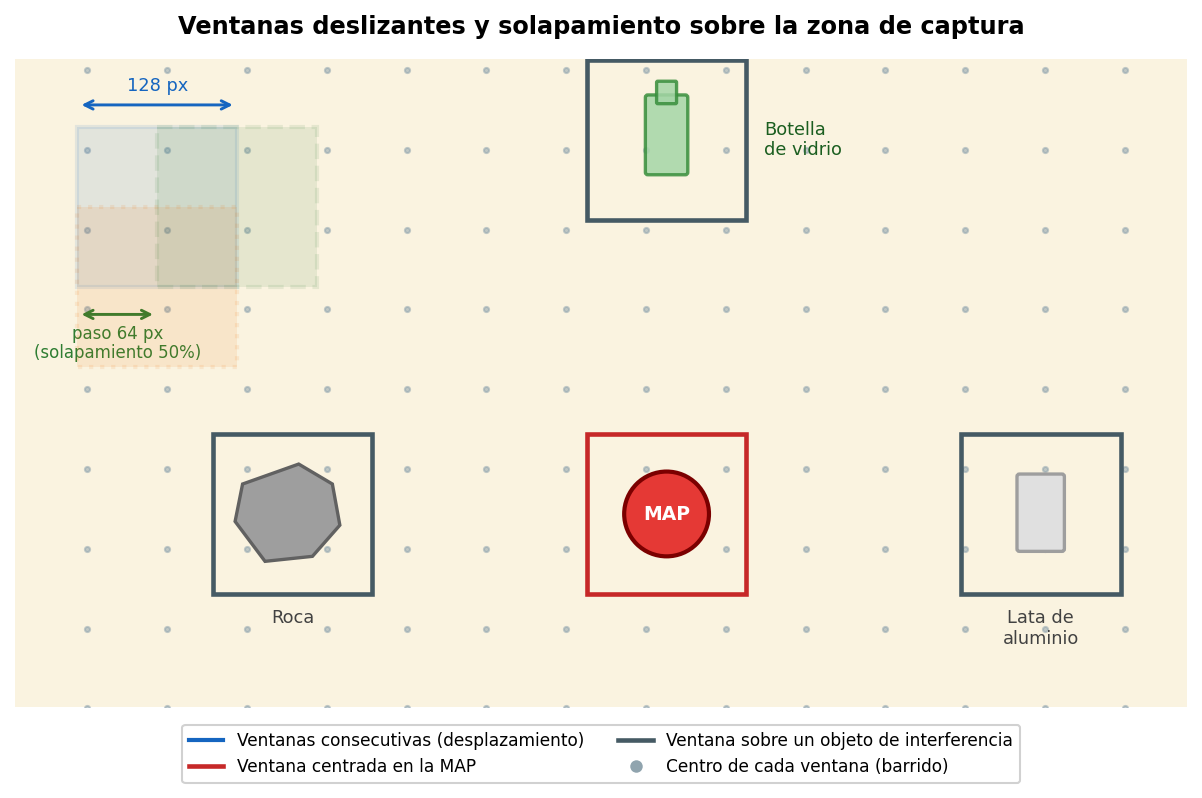
\includegraphics[width=0.92\textwidth]{figuras/ventanas_solapamiento.png}
  \caption{Ventanas deslizantes y solapamiento sobre una zona de captura
    (esquema). Cada ventana de $128\times128$~px se desplaza con un paso
    de 64~px (solapamiento del 50\,\%), de modo que ventanas consecutivas
    comparten la mitad de su área (recuadros de colores). Los puntos marcan
    el centro de cada ventana del barrido completo. La ventana resaltada en
    rojo cubre la \ac{MAP}; cada objeto de interferencia (roca, botella y
    lata) queda cubierto por sus propias ventanas (recuadros grises).}
  \label{fig:ventanas_solapamiento}

  {\footnotesize Fuente: elaboración propia.}
\end{figure}

La etiqueta de cada ventana se asigna ---durante la preparación del conjunto de
entrenamiento--- según la posición de su centro: una ventana es positiva si su
centro cae dentro del bounding box anotado de la \ac{MAP}
(Sección~\ref{sec:segmentacion_groundtruth}), y negativa en caso contrario. Esta
asignación aplica únicamente al groundtruth de entrenamiento; en inferencia, la
ubicación de la mina es desconocida. La Figura~\ref{fig:comparacion_etiquetado}
ilustra el etiquetado sobre una imagen de zona de mina.

\begin{figure}[H]
  \centering
  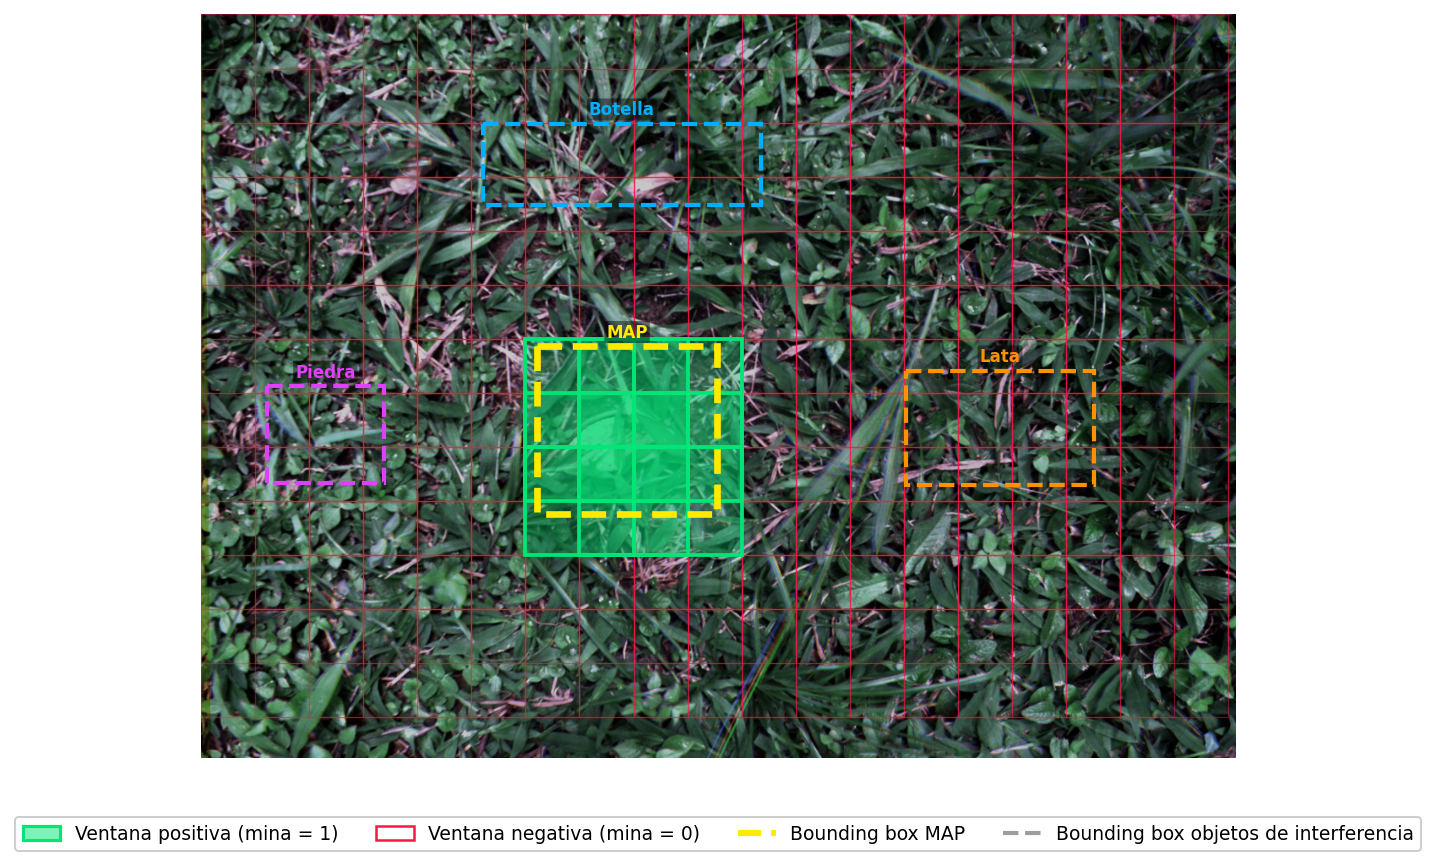
\includegraphics[width=0.7\textwidth]{figuras/comparacion_etiquetado.png}
  \caption{Etiquetado de las ventanas sobre una imagen de zona de mina (S2,
    \texttt{MINA\_7CM\_1}) y la rejilla de ventanas deslizantes
    ($128\times128$~px, paso~64). Cada cuadro representa una ventana; el color
    indica su etiqueta: positiva (verde) si su centro cae dentro del bounding
    box de la \ac{MAP} (rectángulo amarillo discontinuo), y negativa (rojo) en
    caso contrario ---incluidas las ventanas que caen sobre los objetos de
    interferencia (botella, lata y piedra, con su bounding box en color)
    (Sección~\ref{sec:segmentacion_groundtruth}).}
  \label{fig:comparacion_etiquetado}

  {\footnotesize Fuente: elaboración propia.}
\end{figure}

Es importante destacar que el reconocimiento de objetos distintos a la \ac{MAP}
no hace parte de los objetivos de este trabajo. Los objetos de interferencia se
incluyeron para analizar si su presencia puede confundir al sistema y generar
falsas alarmas, como se evalúa en la Sección~\ref{sec:analisis_fp}.

\subsection{Índices espectrales}

Para cada ventana se calculan más de 40 índices espectrales agrupados en tres
categorías: índices de vegetación (NDVI, NDRE, EVI, VARI, entre otros), índices
de suelo (BSI, CI\_soil) e índices de ratio entre bandas (NDRB, Red/Blue,
NIR/Red, y otros). Las ecuaciones de los índices principales se presentaron en
la Sección~\ref{sec:indices_espectrales}.

\subsection{Estadísticas por ventana}

Para cada índice calculado sobre la ventana, se extraen nueve estadísticas de
primer y segundo orden: media, mediana, desviación estándar, mínimo, máximo,
percentiles 25 y 75, asimetría (\textit{skewness}) y curtosis. Con más de 40
índices y 9 estadísticas cada uno, cada ventana queda representada por un vector
de \textbf{378 características}.

% ─────────────────────────────────────────────────────────────
\section{Etapa 2b: Segmentación manual del groundtruth para el aprendizaje supervisado}
\label{sec:segmentacion_groundtruth}

\subsection{Procedimiento de anotación}

Se implementó una etapa de segmentación manual del groundtruth para cada imagen
de zona de mina: se anotó un bounding box sobre la posición exacta del
artefacto, y solo las ventanas cuyo centro cae dentro del bounding box reciben
etiqueta positiva. El etiquetado opera a nivel de ventana (no de píxel), por lo
que la diferencia entre la forma rectangular del bounding box y la sección
circular de la mina tiene un efecto limitado sobre las etiquetas asignadas.

Dado que la mina puede ocupar solo una fracción del área capturada, etiquetar la
zona completa como positiva introduciría ruido: ventanas sin señal de mina
recibirían etiqueta positiva, lo que podría suprimir la contribución de bandas
cuya señal es más sutil y localizada, como el \ac{NIR} y el Red Edge. El
etiquetado preciso por bounding box evita ese ruido.

\subsection{Protocolo de anotación}

En cada sesión de campo se capturan dos imágenes por zona de mina de forma
consecutiva; cada captura corresponde exclusivamente a la zona en cuestión,
sin que otras zonas queden dentro del campo de visión:

\begin{enumerate}
  \item \textbf{Imagen de referencia (UBI):} capturada con el émbolo de la
    jeringa completamente visible sobre la superficie del suelo, lo que
    permite identificar con precisión la posición de la mina en la imagen.
  \item \textbf{Imagen de entrenamiento:} capturada con el émbolo de la
    jeringa cubierto con vegetación natural del entorno, simulando la
    condición real de ocultamiento.
\end{enumerate}

La anotación se realizó en Roboflow usando la composición RGB (bandas 3, 2
y 1) de cada zona como PNG, \textbf{únicamente como interfaz visual} --- la
base de datos se genera del TIF calibrado de 5 bandas, no del PNG. Con la imagen
imagen de referencia, se dibujó un bounding box sobre la región de la mina (clase
\texttt{MAP}) y se exportaron las anotaciones en formato COCO JSON.

\subsection{Transferencia de anotaciones al TIF calibrado}

Las coordenadas del bounding box anotado en la imagen de referencia se
transfieren al TIF calibrado de 5 bandas. Dado que existe un pequeño
desplazamiento entre la imagen de referencia y la imagen de entrenamiento
---capturadas en instantes distintos---, se corrió el algoritmo
\ac{SIFT}+RANSAC directamente sobre la imagen de referencia para registrarla
con la imagen de entrenamiento antes de usar las coordenadas. Lo que se almacena
para el entrenamiento son las coordenadas del bounding box (centro y dimensiones,
en formato COCO JSON), no la imagen de referencia.

Una ventana recibe etiqueta \texttt{tiene\_mina=1} solo si su centro cae dentro
del bounding box; de lo contrario recibe \texttt{tiene\_mina=0}, incluso si
pertenece a una imagen de zona de mina. Con el conjunto de datos completo S2--S7
este etiquetado produjo 487 positivos y 14\,414 negativos (ratio 30:1).


% -------------------------------------------------------------
\section{Etapa 3: Clasificación}

\subsection{Clasificador de desarrollo: Random Forest}
\label{sec:clasificador_rf}

La elección de \ac{RF} se fundamenta en tres propiedades útiles en la etapa
temprana del experimento:

\begin{itemize}
  \item \textbf{Robustez con datos escasos y de alta dimensionalidad.}
    El conjunto de entrenamiento disponible en esta etapa contaba con 487
    ventanas positivas (mina) frente a 378 características, un ratio bajo
    que puede comprometer otros clasificadores. El \ac{RF} maneja bien esta
    condición porque submuestrea características en cada árbol, evitando que
    la alta dimensionalidad domine el ajuste, y no requiere escalado previo
    ni selección manual de variables.
  \item \textbf{Tolerancia al desbalance de clases.} El enfoque de ventana
    deslizante genera de forma inherente un desbalance pronunciado: dado que la
    mina ocupa solo una fracción de la imagen, la mayoría de las ventanas no
    contienen el artefacto --- en la base de datos S2--S7 se obtuvieron
    aproximadamente 30 ventanas negativas por cada positiva. El \ac{RF} tolera
    bien esta condición y, además, el desbalance se corrige de forma explícita
    mediante submuestreo 1:1 al entrenar (Sección~\ref{sec:balanceo}), estrategia
    aplicada por igual a todos los clasificadores comparados.
  \item \textbf{Importancia de características interpretable.} Es posible
    identificar qué estadísticos de índices espectrales son más discriminativos,
    aportando valor diagnóstico independiente de la métrica de exactitud.
\end{itemize}

El modelo se configuró con 100 árboles (\texttt{n\_estimators = 100}),
valor por defecto de scikit-learn que estabiliza las estimaciones de importancia
de características sin costo computacional excesivo; y \texttt{max\_depth = 10},
que limita la profundidad de cada árbol para reducir el sobreajuste con el número
reducido de muestras positivas disponibles. Una vez completada la base de datos
con seis sesiones, se realizó la comparación formal de clasificadores descrita en
la Sección~\ref{sec:comparacion_clasificadores}.



\subsection{Manejo del desbalance de clases}
\label{sec:balanceo}

El etiquetado por bounding box produce 487 ventanas positivas frente a 14\,414
negativas (ratio~30:1). Entrenar directamente sobre esa distribución sesga al
clasificador hacia la clase mayoritaria y degrada la sensibilidad, la métrica más
crítica en este problema. Para corregirlo se aplica \textbf{submuestreo aleatorio
1:1} dentro de cada pliegue de validación: en el conjunto de entrenamiento se
conservan todas las ventanas positivas y se selecciona aleatoriamente un número
igual de ventanas negativas. El submuestreo se realiza \textit{únicamente sobre el
conjunto de entrenamiento de cada pliegue}; la sesión de prueba conserva su
distribución real (30:1), de modo que las métricas se reportan sobre datos no
alterados.

El submuestreo 1:1 descarta una fracción grande de las ventanas negativas
disponibles. Para aprovecharlas sin reintroducir el desbalance, se evalúa
además la estrategia \textbf{EasyEnsemble}: se entrenan diez sub-clasificadores
XGBoost, cada uno con las 487 ventanas positivas y un subconjunto aleatorio distinto
de 487 negativas, y se promedian sus probabilidades. Así cada ventana negativa tiene
oportunidad de participar en el entrenamiento y se reduce la varianza asociada a un
único submuestreo. Esta estrategia ---aplicada por igual durante la comparación de
clasificadores (Sección~\ref{sec:comparacion_clasificadores})--- busca que la
sensibilidad y la especificidad a umbral~0.5 sean representativas, sin requerir
ajuste del umbral.

\subsection{Estrategia de validación LOSO}
\label{sec:loso}

La validación \ac{LOSO}, descrita en la Sección~\ref{sec:loso_teoria}, reserva
en cada iteración $i$ una sesión $i$ completa como prueba y entrena con las
$N-1$ restantes. Las métricas que se empleen durante la búsqueda (AUC, Sensibilidad, Especificidad)
corresponderán al promedio aritmético de los $N$ pliegues.
La Figura~\ref{fig:loso_esquema} ilustra el esquema con los seis pliegues
y garantiza que ninguna ventana de la sesión de prueba aparece durante el entrenamiento.

\begin{figure}[H]
  \centering
  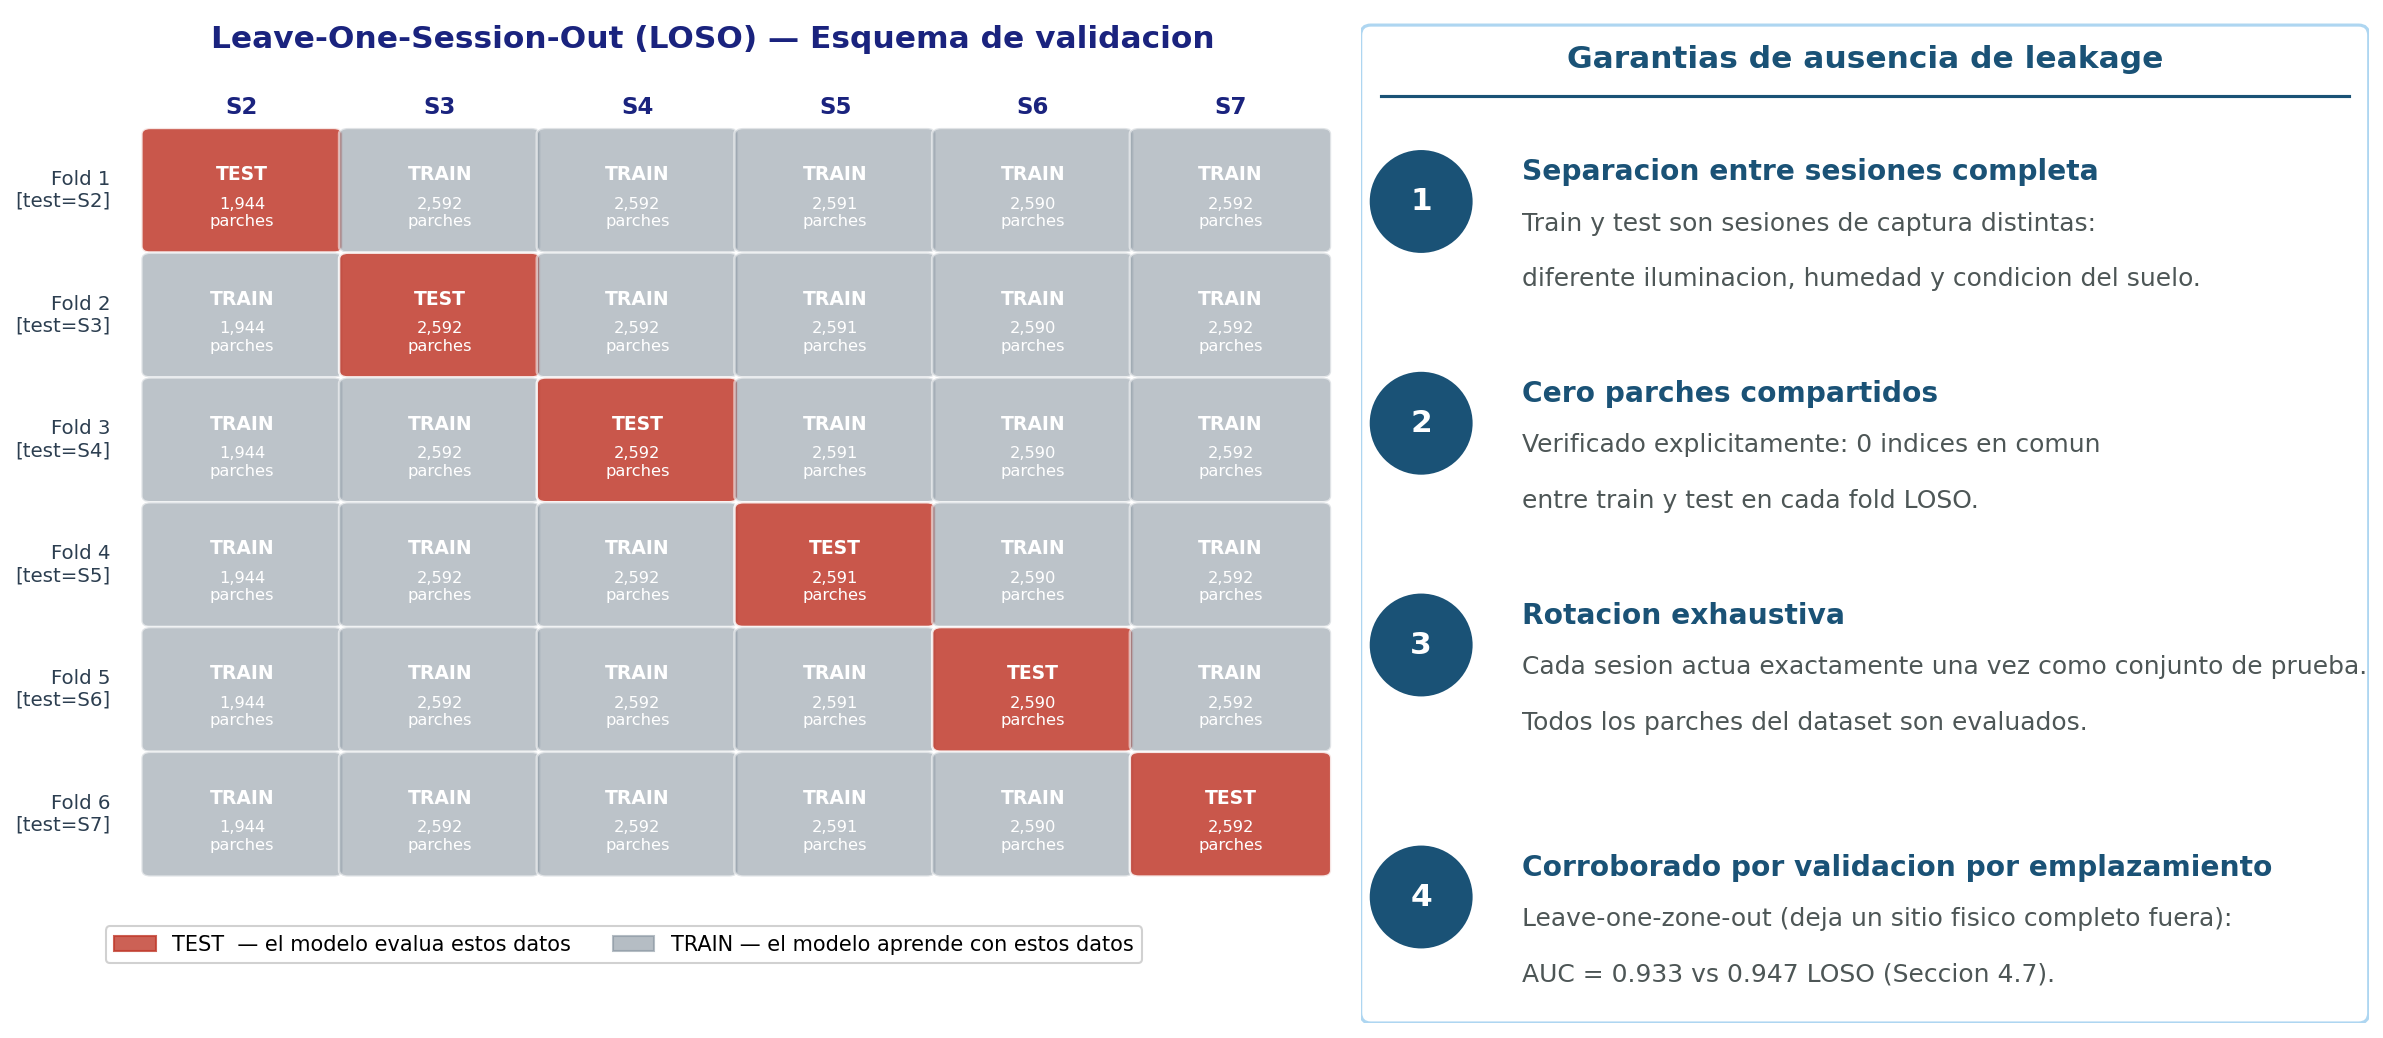
\includegraphics[width=\textwidth]{figuras/loso_justificacion.png}
  \caption{Esquema \ac{LOSO} para seis sesiones (S2--S7): cada fila
    representa un pliegue en que la sesión resaltada en rojo actúa como
    conjunto de prueba y las demás como entrenamiento. El panel derecho
    enumera las garantías de ausencia de fuga de datos, corroboradas por la
    validación por emplazamiento (\textit{leave-one-zone-out}, Sección~\ref{sec:lozo}).}
  \label{fig:loso_esquema}

  {\footnotesize Fuente: elaboración propia.}
\end{figure}

\subsection{Métricas de evaluación}

Se emplean cuatro métricas. El \textbf{AUC} (área bajo la curva \ac{ROC},
independiente del umbral; 0.5 equivale a clasificación aleatoria y 1.0 a
clasificación perfecta) es la métrica principal, pues mide la capacidad
discriminativa sin depender de un umbral y permite comparar configuraciones en
igualdad de condiciones. A umbral fijo~(0.5) se reportan tres métricas operativas:
\textbf{Sensibilidad} (fracción de minas detectadas --- privilegiada por la
asimetría de costos: una mina no detectada es mucho más costosa que una falsa
alarma), \textbf{Especificidad} (fracción de ventanas sin \ac{MAP} correctamente
clasificadas como negativas) y \textbf{falsos positivos por mina} (número de
falsas alarmas por cada mina realmente detectada, indicador del costo operativo de
una eventual inspección). El submuestreo 1:1 descrito en la
Sección~\ref{sec:balanceo} permite que estas tres métricas a umbral~0.5 sean
representativas.


% -------------------------------------------------------------
